\section{Aufbau und Durchführung \cite{sample}}
\subsection{Vorbereitung}
Zur Vorbereitung wurden die Fourierkomponenten von drei verschiedenen periodischen Schwingungsformen
nach den Gleichungen \eqref{eqn:an} und \eqref{eqn:bn} berechnet.
\subsubsection{Rechteck-Spannung}
Eine Rechteckspannung lässt sich durch die Funktion
\begin{equation}
  f(x) =
  \begin{cases}
    -1 , & \text{$-\pi < x < 0$} \\
    1 , & \text{$-0 < x < \pi$} \\
     0, & \text{sonst}
\end{cases}
\end{equation}
beschreiben.
Durch die Gleichungen \eqref{eqn:an} und \eqref{eqn:bn} werden die Fourierkoeffizienten
\begin{align}
  a_n &= 0 \\
  b_n &= \begin{cases}
  0, &\text{n gerade}\\
  \frac{4}{\pi n}, &\text{sonst}
  \end{cases}
\end{align}
bestimmt. Somit lautet, nach \eqref{eqn:FT}, die Fourier-Reihe für eine Rechteck-Spannung:
\begin{equation}
  f_n(x) = \frac{4}{\pi}\sum\limits_{k=1}^{n}\frac{sin{((2k-1)x)}}{2k-1}
\end{equation}

\begin{figure}[H]
  \centering
  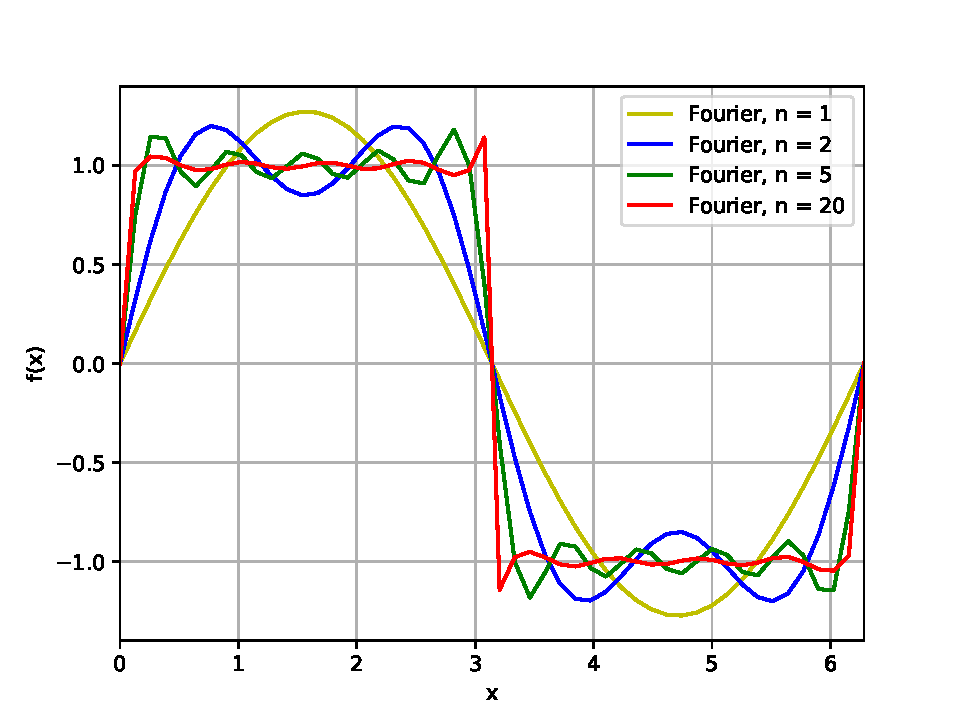
\includegraphics[scale=0.7]{Plots/Fourier/rf.pdf}
  \caption{Näherung der Rechteck-Spannung mithilfe der Fourier-Reihe}
  \label{fig:rf}
\end{figure}
\subsubsection{Sägezahn-Spannung}
Eine Sägezahn-Spannung wird durch die Funktion
\begin{equation}
  f(x) =
  \begin{cases}
    -x , & \text{$-\pi < x < \pi$} \\
     0, & \text{sonst}
\end{cases}
\end{equation}
beschrieben.
Erneut werden durch die Gleichungen \eqref{eqn:an} und \eqref{eqn:bn} die Fourierkoeffizienten bestimmt:
\begin{align}
  a_n &= 0 \\
  b_n &= -2\frac{(-1)^{n+1}}{n}
\end{align}
Somit ist, nach \eqref{eqn:FT} , die Fourier-Reihe für eine Sägezahn-Spannung :
\begin{equation}
  f_n(x) = -2\sum\limits_{k=1}^{n}(-1)^{k+1}\frac{sin{(kx)}}{k}
\end{equation}


\begin{figure}[H]
  \centering
  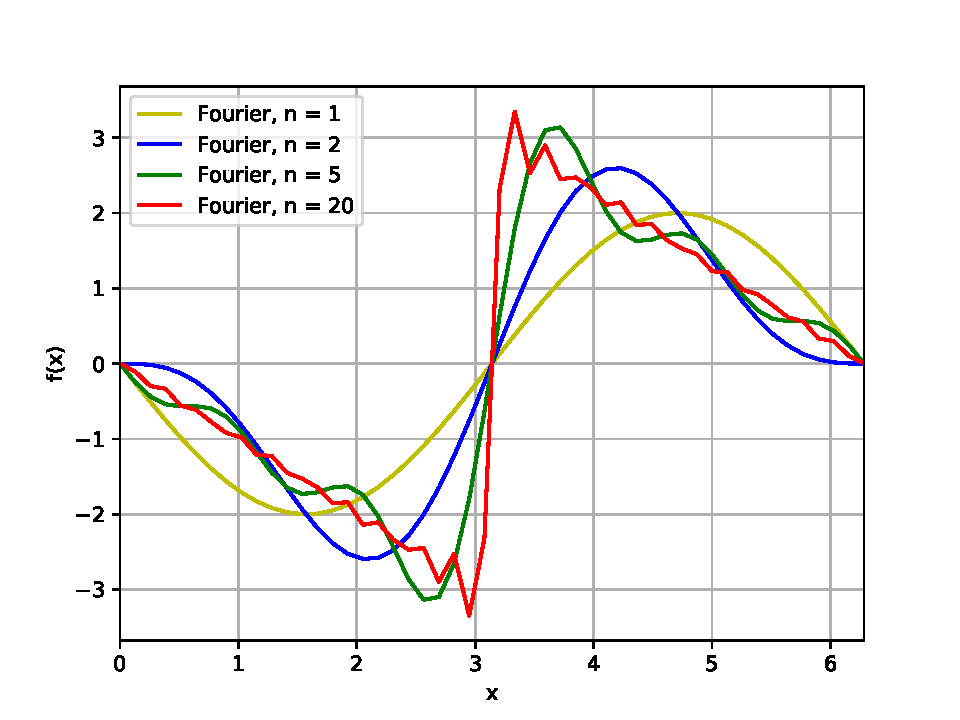
\includegraphics[scale=0.7]{Plots/Fourier/sf.pdf}
  \caption{Näherung der Sägezahn-Spannung mithilfe der Fourier-Reihe}
  \label{fig:sf}
\end{figure}

\subsubsection{Dreieck-Spannung}
Eine Dreieck-Spannung wird durch die Funktion
\begin{equation}
  f(x) =|x| \text{ für $-\pi \le x \le \pi$}
\end{equation}
beschrieben.
Auch hier ergeben sich aus den Gleichungen \eqref{eqn:an} und \eqref{eqn:bn} die Fourierkoeffizienten:


\begin{align}
  a_n &= \begin{cases}
    0 , & \text{n gerade} \\
     -\frac{4}{\pi n^2}, & \text{sonst}
\end{cases}\\
  b_n &= 0
\end{align}
Die Fourier-Reihe für eine Dreieck-Spannung lautet, nach \eqref{eqn:FT}, also:
\begin{equation}
  f_n(x) =\frac{\pi}{2} -\frac{4}{\pi}\sum\limits_{k=1}^{n}(-1)^{k+1}\frac{cos{((2k-1)x))}}{(2k-1)^2}
\end{equation}


\begin{figure}[H]
  \centering
  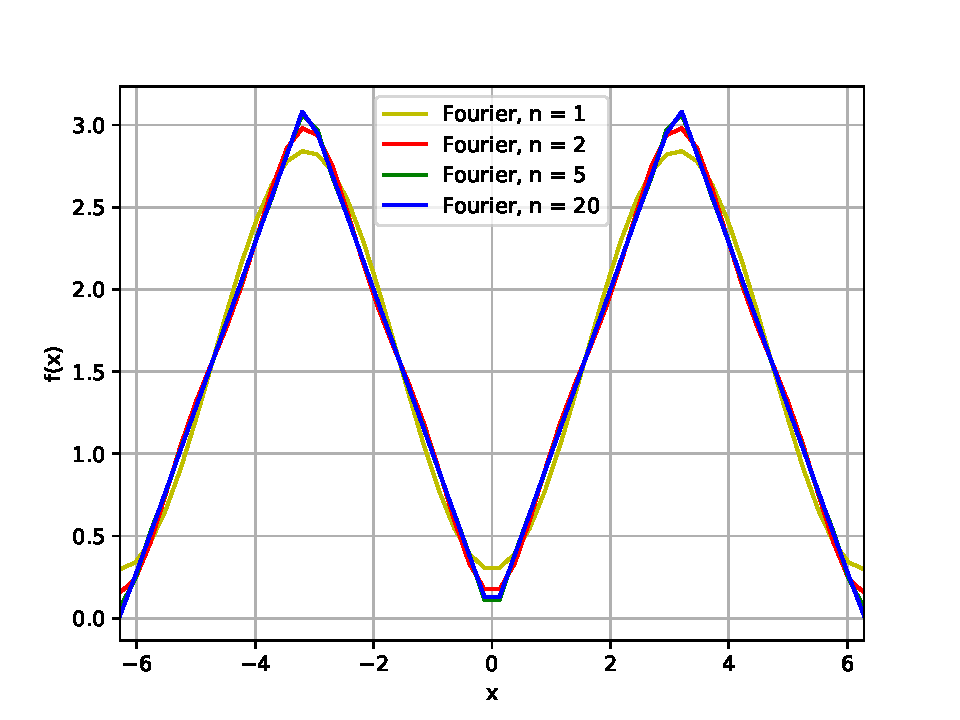
\includegraphics[scale=0.7]{Plots/Fourier/df.pdf}
  \caption{Näherung der Dreieck-Spannung mithilfe der Fourier-Reihe}
  \label{fig:df}
\end{figure}


\subsection{Fourier-Analyse}
Die drei in der Vorbereitung gewählten Schwingungsformen sollen mithilfe der Fourier-Analyse untersucht werden.
Dazu wird ein Funktionsgenerator an ein Oszilloskop angeschlossen.
In diesem Fall wird die Fourier-Transformation automatisch vom Oszilloskop durchgeführt und liefert ein
Linienspektrum wie in Abbildung \ref{fig:linie}. Es werden nun die Amplituden und Frequenzen
der Peaks mithilfe der Cursor-Funktion des Oszilloskops ausgemessen.

\subsection{Fourier-Synthese}
In diesem Teil des Experiments sollen die drei ausgewählten Schwingungsformen mithilfe eines Oberwellengenerators
synthetisiert werden.
Dazu werden zunächst die einzelnen Oberwellen an das Oszilloskop angeschlossen und die Amplituden
entsprechend eingestellt. Dabei wird die Grundfrequenz auf die Maximalspannung gestellt und die restlichen Oberwellen daran
angepasst. Außerdem ist zu beachten, dass bei der Rechteck- und Dreieck-Spannung nur die ungeraden Oberwellen
verwendet werden dürfen.
Im Anschluss wird die Summation aller eingestellten Oberwellen an das Oszilloskop angeschlossen und die
Phasen reguliert, bis die gewünschten Schwingungsformen zu erkennen sind.
